\documentclass[13pt]{article}\usepackage[]{graphicx}\usepackage[]{color}
% maxwidth is the original width if it is less than linewidth
% otherwise use linewidth (to make sure the graphics do not exceed the margin)
\makeatletter
\def\maxwidth{ %
  \ifdim\Gin@nat@width>\linewidth
    \linewidth
  \else
    \Gin@nat@width
  \fi
}
\makeatother

\definecolor{fgcolor}{rgb}{0.345, 0.345, 0.345}
\newcommand{\hlnum}[1]{\textcolor[rgb]{0.686,0.059,0.569}{#1}}%
\newcommand{\hlstr}[1]{\textcolor[rgb]{0.192,0.494,0.8}{#1}}%
\newcommand{\hlcom}[1]{\textcolor[rgb]{0.678,0.584,0.686}{\textit{#1}}}%
\newcommand{\hlopt}[1]{\textcolor[rgb]{0,0,0}{#1}}%
\newcommand{\hlstd}[1]{\textcolor[rgb]{0.345,0.345,0.345}{#1}}%
\newcommand{\hlkwa}[1]{\textcolor[rgb]{0.161,0.373,0.58}{\textbf{#1}}}%
\newcommand{\hlkwb}[1]{\textcolor[rgb]{0.69,0.353,0.396}{#1}}%
\newcommand{\hlkwc}[1]{\textcolor[rgb]{0.333,0.667,0.333}{#1}}%
\newcommand{\hlkwd}[1]{\textcolor[rgb]{0.737,0.353,0.396}{\textbf{#1}}}%
\let\hlipl\hlkwb

\usepackage{framed}
\makeatletter
\newenvironment{kframe}{%
 \def\at@end@of@kframe{}%
 \ifinner\ifhmode%
  \def\at@end@of@kframe{\end{minipage}}%
  \begin{minipage}{\columnwidth}%
 \fi\fi%
 \def\FrameCommand##1{\hskip\@totalleftmargin \hskip-\fboxsep
 \colorbox{shadecolor}{##1}\hskip-\fboxsep
     % There is no \\@totalrightmargin, so:
     \hskip-\linewidth \hskip-\@totalleftmargin \hskip\columnwidth}%
 \MakeFramed {\advance\hsize-\width
   \@totalleftmargin\z@ \linewidth\hsize
   \@setminipage}}%
 {\par\unskip\endMakeFramed%
 \at@end@of@kframe}
\makeatother

\definecolor{shadecolor}{rgb}{.97, .97, .97}
\definecolor{messagecolor}{rgb}{0, 0, 0}
\definecolor{warningcolor}{rgb}{1, 0, 1}
\definecolor{errorcolor}{rgb}{1, 0, 0}
\newenvironment{knitrout}{}{} % an empty environment to be redefined in TeX

\usepackage{alltt}
\pagestyle{empty}

\usepackage{amsmath}
\usepackage{hyperref}
\usepackage{url}
\usepackage{graphicx}
\usepackage{geometry}
\geometry{verbose,tmargin=0.5in,bmargin=1in,lmargin=1in,rmargin=1in}
\usepackage[version=4]{mhchem}
\IfFileExists{upquote.sty}{\usepackage{upquote}}{}
\begin{document}

%     {\Large{\bf{Name: }}}
%    \begin{center} {\Huge{Quiz 1}}\\ \Large{August 31, 2011} \end{center}
%    No calculators. Show all work.

\textbf{\Large Final Exam }\hfill{}\textbf{DS 210, Spring 2020}

\vspace{0.25in}


Due Date: Wednesday May 20, 2020 by 5:00PM

\vspace{0.25in}

\begin{figure}[h!]
  \centering
  % Requires \usepackage{graphicx}
  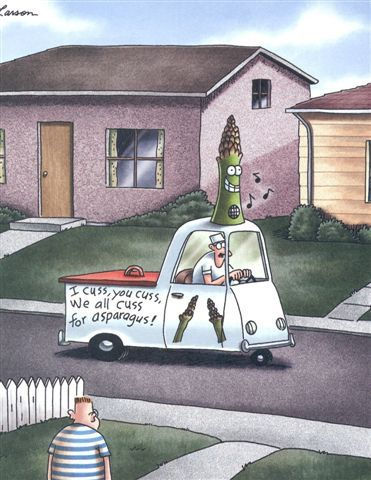
\includegraphics[width=4in]{asparagus.jpg}\\
  %\caption{}\label{}
\end{figure}

\vspace{0.25in}

\begin{quote}
  \Large{I ordered a chicken and an egg from Amazon. I'll let you know.}
\end{quote}

\vspace{0.5in}

{\Large{\bf Read the problems carefully. Show all of your work in a clear, organized manner. You should not seek or receive help on this exam from any individual other than Dr.\ Graham. }}

\newpage

\Large{
    \begin{enumerate}
      \item ({\bf 10 pts.}) Let
    \[ {\bf F} = \left[\begin{array}{ccc} -2 & 1 & 4 \\ -2 &  0 & 2 \end{array}\right]  \]
      and
    \[ {\bf G} = \left[\begin{array}{ccc} 2 & -1 & -3 \\ -6 & 1 & 8 \end{array}\right]  \]
    Compute the following:
    \begin{enumerate}
        \item ${\bf F + G}$
        \item ${\bf F - G}$
        \item ${\bf G - F}$
        \item $2{\bf F}$
        \item $3{\bf G}$
        \item $-4{\bf G}$
        \item $2{\bf F} + 3{\bf G}$
        \item $2{\bf F} - 4{\bf G}$
    \end{enumerate}
    
    \newpage 
    
    \item ({\bf 10 pts.}) Let
    \[ {\bf A} = \left[\begin{array}{ccc} -3 & 1 & 4 \\ -2 &  0 & 2 \end{array}\right]  \]
    \[ {\bf B} = \left[\begin{array}{cc} 2 & -1 \\ -6 & 5 \\ 0 & -1 \end{array}\right]  \]
    and
    \[ {\bf C} = \left[\begin{array}{ccc} 2 & 5 & -1\\ -6 & 1 & 1 \\1 & 0 & -1 \end{array}\right]  \]
    Compute the following expressions or explain why the expression can not be computed. 
    \begin{enumerate}
        \item ${\bf AB}$
        \item ${\bf BA}$
        \item ${\bf AC}$
        \item ${\bf CA}$
        \item ${\bf BC}$
        \item ${\bf CB}$
        \item $({\bf AB}){\bf C}$
        \item ${\bf A}({\bf BC})$
        \item $({\bf CA}){\bf B}$
        \item ${\bf C}({\bf AB})$
        \item ${\bf ACB}$
    \end{enumerate}
    
    \newpage 
    
  \item ({\bf 10 pts.}) For each of the given pairs of matrices, compute ${\bf A}^{T}{\bf B}$ and ${\bf A}{\bf B}^{T}$ whenever possible. 
  
  \begin{enumerate}
      \item 
      \[ {\bf A} = \left[\begin{array}{c} -1 \\ 2 \\ 3 \end{array} \right], \ \ \ {\bf B} = \left[\begin{array}{c} -1 \\ 0 \\ 2 \end{array} \right] \]
      \item 
      \[ {\bf A} = \left[\begin{array}{ccc} -2 & 1 & -3 \end{array} \right], \ \ \ {\bf B} = \left[\begin{array}{ccc} -1 & 0 & 2 \end{array} \right] \]
      \item 
      \[ {\bf A} = \left[\begin{array}{ccc} -2 & 1 & 3 \end{array} \right], \ \ \ {\bf B} = \left[\begin{array}{ccc} 1 & 0 & 2 \\ 1 & 0 & -1 \end{array} \right] \]
      \item 
      \[ {\bf A} = \left[\begin{array}{ccc} -2 & 1 & 3 \\ 2 & 1 & -1 \end{array} \right], \ \ \ {\bf B} = \left[\begin{array}{ccc} -1 & 0 & 2 \end{array} \right] \]
      \item 
      \[ {\bf A} = \left[\begin{array}{ccc} -2 & 1 & 3 \\ 2 & 1 & -1 \end{array} \right], \ \ \ {\bf B} = \left[\begin{array}{ccc} -1 & 0 & 2 \\ 1 & 0 & -1 \end{array} \right]\]
      \item 
      \[ {\bf A} = \left[\begin{array}{ccc} -2 & 1 & 3 \\ 2 & 1 & -1 \\ 5 & 1 & 7 \end{array} \right], \ \ \ {\bf B} = \left[\begin{array}{ccc} -1 & 0 & 2 \end{array} \right] \]
      \item 
      \[ {\bf A} = \left[\begin{array}{ccc} 2 & 1 & -3 \\ 2 & 1 & -1 \\ -4 & 6 & 10 \end{array} \right], \ \ \ {\bf B} = \left[\begin{array}{ccc} -1 & 0 & 2 \\ 1 & 0 & -1 \\ -1 & -1 & -1 \end{array} \right]\]
  \end{enumerate}
  
  \newpage
  
  \item ({\bf 10 pts.}) Find the inverse matrix for each of the following $2\times 2$ matrices.  
    \begin{enumerate}
      \item 
      \[ {\bf A} = \left[\begin{array}{cc} 1 & -1 \\ -2 & 4  \end{array} \right] \]
       \item 
      \[ {\bf A} = \left[\begin{array}{cc} -1 & 0 \\ -2 & -4  \end{array} \right] \]
       \item 
      \[ {\bf A} = \left[\begin{array}{cc} 2 & -1 \\ -2 & 1  \end{array} \right] \]
       \item 
      \[ {\bf A} = \left[\begin{array}{cc} 3 & 2 \\ 4 & -1  \end{array} \right] \]
  \end{enumerate}
  
  \newpage
  
  \item ({\bf 5 pts.})  Use R to compute the {\bf determinant} of the given matrix. 
 \[ {\bf A} = \left[\begin{array}{ccc} 2 & 1 & -3 \\ -2 & 1 & -1 \\ 5 & 1 & 7 \end{array} \right]\]
 
 \vspace{2.5in}
 
 \item ({\bf 5 pts.}) Use R to compute the {\bf inverse} of the given matrix. 
 \[ {\bf A} = \left[\begin{array}{ccc} -2 & -1 & 3 \\ 2 & 1 & -1 \\ 5 & 1 & -7 \end{array} \right]\]
 Verify that you have obtained the correct answer. 
 
 \newpage 
 
 \item ({\bf 5 pts.}) Use R to obtain a plot of the plane corresponding to the two variable linear function $F(x_{1},x_{2}) = 3x_{1} - 5x_{2} - 2$.
 
 \vspace{2.5in}
 
\item ({\bf 5 pts.}) Use R to obtain a contour plot for the two variable function $F(x_{1},x_{2}) = \cos(x_{1}^{2} - x_{2}^{2})$. 

\newpage

\item ({\bf 10 pts.}) Find all first partial derivatives for each of the given functions.
  \begin{enumerate}
       \item $F(x_{1},x_{2}) = x_{1}e^{3x_{2}}$
        \item $F(x_{1},x_{2}) = \frac{x_{1} - x_{2}}{x_{1} + x_{2}}$
          \item $F(x_{1},x_{2},x_{3}) = x_{1}x_{2}^{2}x_{3}^{3} + 3x_{2}x_{3}$
           \item $F(x_{1},x_{2},x_{3}) = x_{1}x_{2} - x_{1}x_{3} + x_{2}x_{3}^{4}$
            \item $F(x_{1},x_{2},x_{3}) = x_{1}\cos(x_{2}) + x_{2}\sin(x_{3})$
  \end{enumerate}
  
  \newpage
  
  \item ({\bf 10 pts.}) Let $F(x_{1},x_{2}) = 3x_{1}^4 - 4x_{1}x_{2} + x_{2}^{2} + 1$. 
  \begin{enumerate}
      \item Find an equation for the plane tangent to the graph of the function at the point $(-1,2)$.
  \end{enumerate}
  
  \vspace{2.5in}
  
   \item ({\bf 10 pts.})  Let $F(x_{1},x_{2}) = 4x_{1}^2 x_{2} - 7x_{1} x_{2}^2 - 2x_{2}^{3} + 5$ and let $x_{1}(u,v) = 2uv$ and $x_{2}(u,v) = u-v$. Use the multivariable chain rule to compute the partial derivatives $\frac{\partial G}{\partial u}$ and $\frac{\partial G}{\partial v}$, where $G(t) = F(x_{1}(u,v),x_{2}(u,v))$.
   
   \newpage 
   
    \item ({\bf 10 pts.})  Find the critical points of the following functions. Use the second derivative test to determine (if possible) whether each critical point corresponds to a local maximum, local minimum, or saddle point. 
  \begin{enumerate}
      \item $F(x_{1},x_{2}) = 4 + 2x_{1}^{2} + 3x_{2}^{2}$
      \item $F(x_{1},x_{2}) = -4x_{1}^{2}+8x_{2}^{2} - 3$
      \item $F(x_{1},x_{2}) = x_{1}^{4} + 2x_{2}^{2} - 4x_{1}x_{2}$
  \end{enumerate}
  
  \newpage
  
  \item ({\bf 5 pts.}) Suppose we roll three fair six-sided dice. Compute the probability that the sum is
  \begin{enumerate}
      \item 4
      \item 8
  \end{enumerate}
  
  \vspace{2.5in}
  
  \item  ({\bf 5 pts.}) A friend flips two fair coins and tells you that at least one is heads. Given this information, what is the probability that the first coin in heads? 
  
  \newpage 
  
  \item ({\bf 5 pts.}) 5\% of men and 0.25\% of women are color blind. Assuming that there are an equal number of men and women, what is the probability that a color-blind person is a man?
  
  \vspace{2.5in}
  
  \item ({\bf 5 pts.}) Suppose we randomly select one of five numbers with the following probabilities: 1 with probability $\frac{1}{14}$, 2 with probability $\frac{1}{7}$, 3 with probability $\frac{3}{14}$, 4 with probability $\frac{2}{7}$, 5 with probability $\frac{2}{7}$. Let $X$ be the random variable that returns the chosen number. Calculate the following values:
  \begin{enumerate}
      \item $P(X \leq 3)$
      \item $P(X > 3)$
      \item $P(X < 4.12 )$
  \end{enumerate}
  
  \newpage 
  
  \item ({\bf 10 pts.})  Let $X$ be a continuous random variable with probability density function (pdf)
  \[ f(x) = \left\{\begin{array}{ll} 5e^{-5x}, & \mbox{if $x > 0$,} \\ 0, & \mbox{else.}  \end{array} \right.  \]
  \begin{enumerate}
      \item Verify that 
      \[ \int_{-\infty}^{\infty}f(x) \ dx = 1. \]
      \item Compute $P(-1 < X < 1)$.
      \item Compute $P(X \leq 5)$.
      \item Determine the cumulative distribution function (cdf) $F$ for $X$.  
      \item Compute the expected value $E[X]$.
      \item Compute $E[e^{3X}]$.
  \end{enumerate}
  
  \newpage
  
  \item ({\bf 10 pts.}) Suppose that $X$ is a binomial random variable with $n=20$ and probability of success $\rho = \frac{3}{4}$. 
  \begin{enumerate}
      \item Compute $E[X]$. 
      \item Compute $\text{Var}[X]$.
      \item Use R to plot the pmf of $X$. 
      \item Compute the following probability values (you can use R to do this):
      \begin{enumerate}
          \item $P(X = 3)$
          \item $P(X = 5)$
          \item $P(X \leq 5)$
          \item $P(2 \leq X \leq 7 )$
          \item $P(2 < X < 7)$
          \item $P(x > 3)$
      \end{enumerate}
  \end{enumerate}
  
  \newpage
  
  \item ({\bf 10 pts.}) Suppose that the random variable $X$ has expected value $E[X] = 4$ and variance $\text{Var}[X] = 9$. Compute the following quantities:
  \begin{enumerate}
      \item $E[3X+2]$
      \item $E[X^2]$
      \item $E[(2X+3)^2]$
      \item $\text{Var}[4X - 2]$
  \end{enumerate}
    
    
\newpage

\item ({\bf 10 pts.}) Let $X$ be a normal random variable with mean $\mu = -2$ and variance $\sigma^2 = 4$. 
  \begin{enumerate}
      \item Find the probability $P(2 < X < 6)$.
      \item Find $E[X^2]$. 
  \end{enumerate}
  
  \newpage 
  
  \item ({\bf 10 pts.})  Consider the flight delays data from the {\tt resample} package, the first few rows of the relevant columns are shown below
\begin{knitrout}
\definecolor{shadecolor}{rgb}{0.969, 0.969, 0.969}\color{fgcolor}\begin{kframe}
\begin{alltt}
\hlkwd{head}\hlstd{(FlightDelays[,}\hlkwd{c}\hlstd{(}\hlstr{"Carrier"}\hlstd{,}\hlstr{"Delay"}\hlstd{)])}
\end{alltt}
\begin{verbatim}
##   Carrier Delay
## 1      UA    -1
## 2      UA   102
## 3      UA     4
## 4      UA    -2
## 5      UA    -3
## 6      UA     0
\end{verbatim}
\end{kframe}
\end{knitrout}
  Notice that the data contains flight delays for two airlines, American and United. 

  \begin{enumerate}
  \item Compute the proportion of times that each carrier's flights was delayed more than 20 minutes. Conduct a two-sided permutation test to see if the     difference in these proportions is statistically significant. 
  \end{enumerate}

\newpage 

\item ({\bf 10 pts.}) Consider the Bangladesh data set from the {\tt resampledata} package:
\begin{knitrout}
\definecolor{shadecolor}{rgb}{0.969, 0.969, 0.969}\color{fgcolor}\begin{kframe}
\begin{alltt}
\hlkwd{head}\hlstd{(Bangladesh)}
\end{alltt}
\begin{verbatim}
##   Arsenic Chlorine Cobalt
## 1    2400      6.2   0.42
## 2       6    116.0   0.45
## 3     904     14.8   0.63
## 4     321     35.9   0.68
## 5    1280     18.9   0.58
## 6     151      7.8   0.35
\end{verbatim}
\end{kframe}
\end{knitrout}
This data records levels of three chemicals found in the groundwater of Bangladesh. In this problem we will use the bootstrap to understand the distribution of levels of cobalt (measured in parts per billion (ppb)) in the groundwater. We can extract the vector of cobalt levels as follows:
\begin{knitrout}
\definecolor{shadecolor}{rgb}{0.969, 0.969, 0.969}\color{fgcolor}\begin{kframe}
\begin{alltt}
\hlstd{Cobalt} \hlkwb{<-} \hlstd{Bangladesh}\hlopt{$}\hlstd{Cobalt}
\end{alltt}
\end{kframe}
\end{knitrout}

\begin{enumerate}
\item  Compute the mean and standard deviation for the cobalt level recorded in the Cobalt data. 

\item Use 10,000 resamples to compute the bootstrap distribution for the sample mean of the Cobalt data. 

\item  Plot a histogram of the bootstrap distribution. 

\item  Use the boostrap to find and interpret an approximate 95\% confidence interval for the sample mean of the Cobalt data. 
\end{enumerate}
    
    \end{enumerate}


\end{document}
